\documentclass[a4paper,12pt]{article}

\usepackage[latin1]{inputenc} % accents
\usepackage[T1]{fontenc}      % caract�res fran�ais
\usepackage{geometry}         % marges
\usepackage{lmodern}
\usepackage[french]{babel}
\usepackage{url,csquotes}
\usepackage[hidelinks,hyperfootnotes=false]{hyperref}
\usepackage{graphicx}
\usepackage[titlepage]{polytechnique}
\usepackage{textcomp}
\usepackage{float}
\usepackage{enumerate}
\usepackage{enumitem}%textbullets
 \frenchbsetup{StandardLists=true}%textbullets
 \usepackage{soul}
 \usepackage{color}
 \usepackage{amsfonts}
 
 
\title{Low Dimensional Embedding of Environmental Variables}      % renseigne le titre
\subtitle{EA MAP581}
\author{Flore Martin and Lorraine Roulier}           %   "   "   l'auteur
%\date{\today}           %   "   "   la future date de parution
\renewcommand{\thesection}{\arabic{section}}

\definecolor{bleu}{rgb}{0.5, 1.0, 1.0}
\newcommand{\hlb}[1]{\sethlcolor{bleu}\hl{#1}}


\begin{document}

\maketitle
\tableofcontents
\newpage

\section{Introduction}

Climate data amounts very quickly to a lot of unused data. In a day, we can collect temperature, pressure, wind data all over the world with satellites, even hourly. Our project was two sided. First, we familiarized with various dimension reduction techniques, then we attempted to show that the geographical position of a point on the planet - e.g. it's latitude and longitude - were embedded in the climate data one could gather on it. 

Dimension reduction techniques can be divided in two classes, linear dimension reduction and non linear dimension reduction. However, in all methods, the main goal is to figure out a similarity function between vectors. Such a function will then enable to sort the dataset into classes of vectors with similar features, which would have been more intricate with the initial dataset. 
We used a set of datasets we found on the NASA website, that gathered various means on climate variables over 22 years at every given latitude and longitude. These variables are gathered in the table below

\begin{figure}[H]
 \begin{center}
	
	\begin{tabular}{|c|c|c|c|c|c|c|}
		 \hline    
	  	Latitude & Longitude &Temperature & Pressure&  Relative Humidity& Wind Speed& Radiation\\ 
		
		& & �$C$ & $kPa$ & $ \%$ & $m/s$ & $kWh/m^{2}/day$ \\ 
		\hline
		  \end{tabular}
\end{center}
\caption{First lign of our dataset}
\end{figure}

The latitude parameter varies from -90 to 89 and the longitude parameter varies from -180 to 179. the negative values are for the south hemisphere, the positive ones for the north. Depending on the running time of the method, we did not compute the dimension reduction with the 64800 lines, but with a subset. 
The subset is often a slice of longitudes containing all latitudes, as we assumed that the critical parameter to differenciate climate data was the latitude. 

\begin{figure}[H]
 \begin{center}
	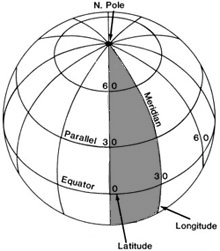
\includegraphics[scale = 4]{latlon.jpg}
\end{center}
\caption{An example of subset in grey}
\end{figure}

\section{Principal Component Analysis - PCA}
	\subsection{Method}
	
		Principal Component Analysis detects tendencies in the data by maximizing the variance of the dataset matrix. This yields an orthonormal matrix that can be diagonalized. The largest eigenvalues point to the eigenvectors that contain the most information about the dataset. 
		
		Let $ X \in \mathbb{R}^{d \times n} $ be our dataset, PCA maximizes the following equation :
%%
\[ \| X - MM^{T}X \|^{2} \]
subject to $ M \in \mathcal{O}^{d \times r} $ where $ r<d $.

	\subsection{Results}
		\subsubsection{Two dimensions}
		
		We first implemented PCA and ran it with only two principal components
\section{Kernel Principal Component Analysis}
	\subsection{Method}
	\subsection{Results}
\section{Multidimensional Scaling - MDS}
	\subsection{Method}
	\subsection{Results}
\section{Isomap}
	\subsection{Method}
	\subsection{Results}
\section{Comparing the different methods}
\section{Conclusion}
\section{Bibliography}


\end{document}
